% Prof. Dr. Ausberto S. Castro Vera
% UENF - CCT - LCMAT - Curso de Ci\^{e}ncia da Computa\c{c}\~{a}o
% Campos, RJ,  2022
% Disciplina: Paradigma de Desenvolvimento Orientado a Objetos
% Aluno:


\chapterimage{conclusoes.png} % Table of contents headi ng image
\chapter{Considera\c{c}\~{o}es Finais}


O trabalho desenvolvido se trata de um sistema que permite ao usuário criar atividades em uma agenda e compartilhar com seus colegas de empresa.
Este trabalho teve como objetivo desenvolver um sistema que aplique os conhecimentos adquiridos no curso para obtenção de nota de crédito na disciplina de paradigma orientado a objetos para desenvolvimento de software, além de recordar os conceitos das disciplinas do curso de Ciência da Computação.
. Entre os problemas encontrados na realização do trabalho, o mais importante foi o desenvolvimento da parte escrita. No entanto, essas dificuldades contribuem para o desenvolvimento de soft skills e competências técnicas necessárias no mercado de trabalho, tais como: Compreensão da demanda de trabalho, priorização, gestão do tempo. Os aspectos não considerados úteis para o sistema seriam: o desenvolvimento de uma interface para o cliente onde pudesse haver uma criação de atividade para que o gerenciamento das tarefas dos funcionários da empresa; configurar uma página exclusiva para pessoas de fora da empresa.

Recursos a serem desenvolvidos no futuro:
\begin{itemize}
    \item  Troca de mensagens entre o usuário e o criador da atividade na agenda;
    \item  Favoritos: O sistema permitirá que os usuários possam marcar as propriedades que deseja adicionar aos favoritos.
    \item  Editar informações do usuário: bem como recurso favorito, o sistema possuirá personalização para que o usuário possa modificar as informações do usuário.

\end{itemize}



\begin{figure}[H]
    \begin{center}
        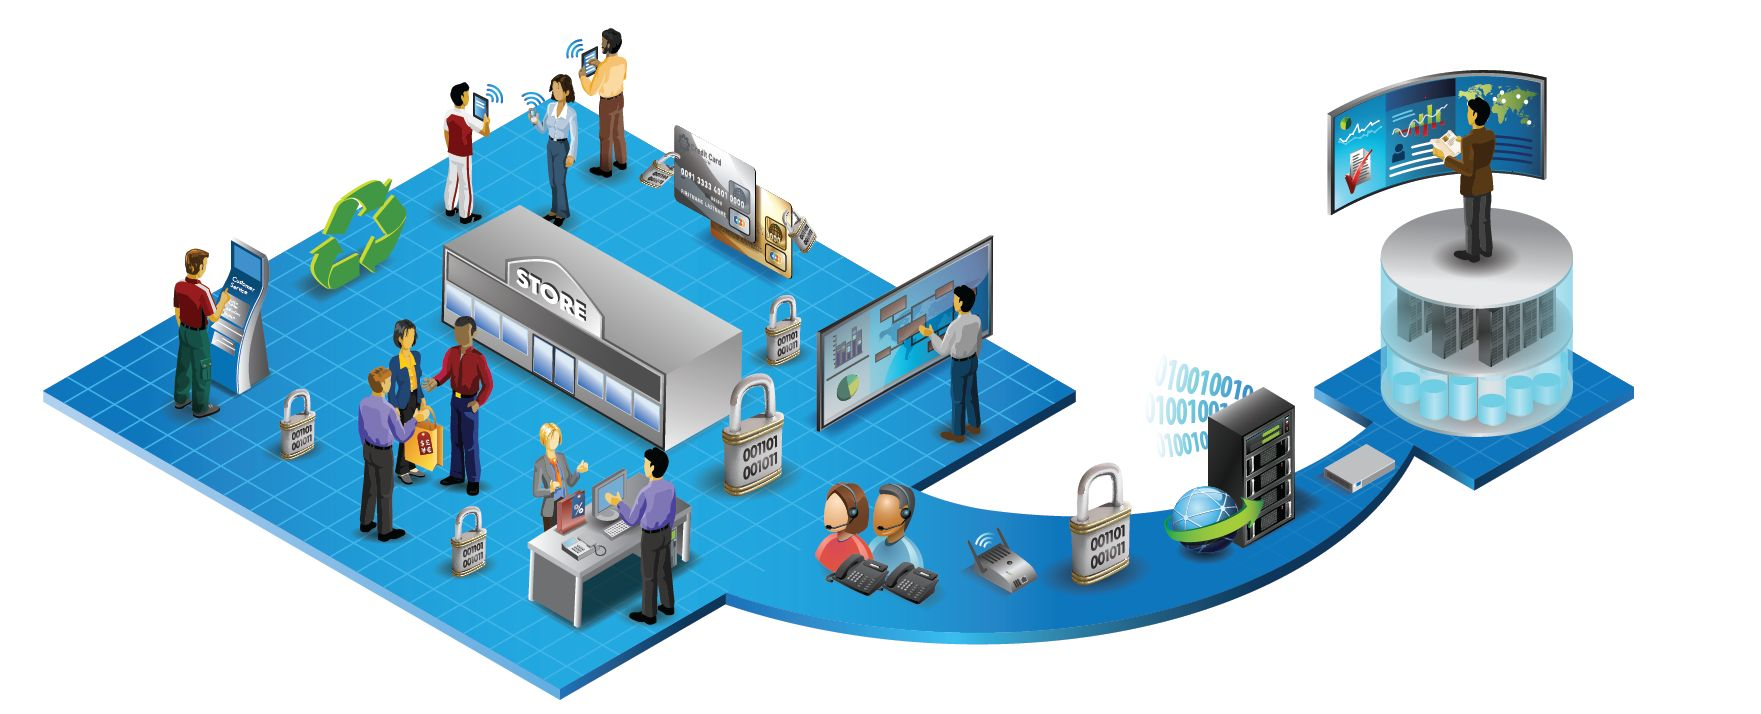
\includegraphics[width=12cm]{MeuSistema.jpg}
        \caption{Meu Sistema a ser desenvolvido} \label{sistema}
    \end{center}
\end{figure}
